\section{Monday 09/23/2024}

\subsection{KKT Condition qualification}
Drawing out the problem
\begin{equation}
  \begin{aligned}
    min -x_1 \\
    s.t. x_2 - (1-x_1)^3 \leq 0 \\
    x_1 \geq 0, x_2 \geq 0 
  \end{aligned}
\end{equation}

\begin{figure}[htbp]
  \centerline{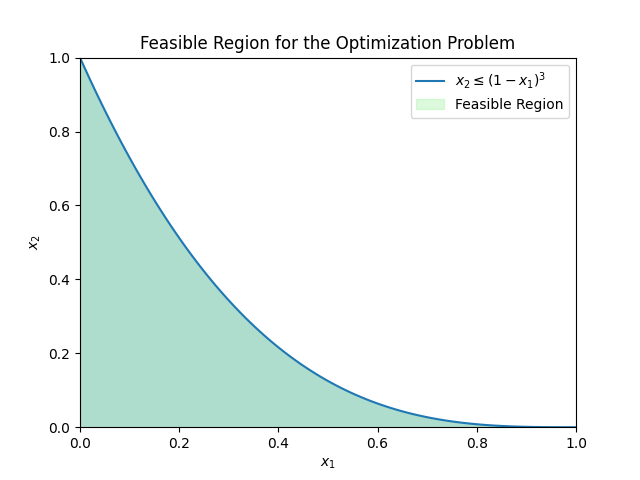
\includegraphics[width=0.75\textwidth]{images/kkt_feasible_region.png}}
  \caption{Graph of the feasible region of the problem above}
  \label{fig:kkt_feasible_region}
\end{figure}

The objective function is minimized at the point (1,0). To be rigorous, we check if this optimization problem satisfies the KKT conditions.
\begin{align}
  \text{Stationary condition: }
  \begin{bmatrix}
     -1 \\
     0
  \end{bmatrix}
  + 
  \gamma_1
  \begin{bmatrix}
    -3(1-x_1)^2\\
    1
 \end{bmatrix}
 -
 \gamma_2
 \begin{bmatrix}
  1 \\
  0
 \end{bmatrix}
 -
 \gamma_3
 \begin{bmatrix}
  0 \\
  1
 \end{bmatrix}
 = 0
\end{align}
This stationary condition is not true when $x_1, x_2 = (1,0)$ because each $\gamma_i \geq 0$. There are no non-negative $\gamma_i$ that satisfy the stationary condition.  
\\ \\
\subsection{Adding regularity condition}
\begin{itemize}
  \item Linear CQ: $g$ and $h$ are affine functions
  \item Linear indendepence CQ: The gradients of the active inequality constraints and the gradients of the equality constraints are linearly independent.
\end{itemize}
Only one of the above constraint qualifications should hold to allow the KKT conditions to work. For the previous example, since the objective function is cubic, the KKT conditions do not hold. The conditions are also solution specific.

\subsection{Fritz John conditions}
The Fritz John conditions are a slight modification to the KKT conditions

\framebox[\linewidth]{
    \begin{minipage}{\dimexpr\linewidth-2\fboxsep-2\fboxrule\relax}
      \begin{equation}
        \begin{aligned}
          \lambda \nabla f(x^*) + [\nabla h(x^*)]^T \Theta + [\nabla g(x^*)]^T \Gamma = 0, \\
          [g(x^*)]^T\Gamma = 0, \\
          \lambda \geq 0, \Gamma \geq 0, \\
          h(x^*) = 0, g(x^*) \leq 0
        \end{aligned}
      \end{equation}
    \end{minipage}
}

There is an introduction of the $\lambda$ coefficient to the objective function that alleviates the regularity conditions to the KKT conditions. 

\subsection{NLP: Part III}
Convex sets and functions. \\ \\
\framebox[\linewidth]{
    \begin{minipage}{\dimexpr\linewidth-2\fboxsep-2\fboxrule\relax}
        A function $h: \mathbb{R}^n \to \mathbb{R}$ is said to be convex if and only if it satisfies 
        \begin{equation}
          \lambda h(x_1) + (1-\lambda)h(x_2) \geq h(\lambda x_1 + (1-\lambda)x_2)
        \end{equation}  
        for any $\lambda \in [0,1]$ and any $x_1, x_2 \in \textbf{dom } h$ 
    \end{minipage}
}
\\ \\ 
\framebox[\linewidth]{
    \begin{minipage}{\dimexpr\linewidth-2\fboxsep-2\fboxrule\relax}
        A set $\Omega \subseteq \mathbb{R}^n $ is said to be convex if and only if it satisfies 
        \begin{equation}
          \lambda x_1 + (1-\lambda)x_2 \in \Omega
        \end{equation}  
        for any $\lambda \in [0,1]$ and any $x_1, x_2 \in \Omega$ 
    \end{minipage}
}
